\documentclass[a4paper]{article}
\usepackage[utf8]{inputenc}
\usepackage[T1]{fontenc}
\usepackage[french]{babel}
\usepackage{amsmath,amssymb}
\usepackage{amsfonts}
\usepackage{amssymb}
\usepackage{amsthm}
\usepackage{lmodern}
\usepackage{color}
\usepackage{graphicx}
\usepackage{geometry}
\usepackage{dialogue}


\def\dsum{\sum\limits}
\def\dint{\displaystyle\int}
\def\ie{\leqslant}
\def\C{\mathbb{C}}
 \parskip 5mm
 \parindent 5mm
 \definecolor{Green}{RGB}{20,200,50}
 \definecolor{Red}{RGB}{200,50,20}
 \definecolor{Blue}{RGB}{50,20,200}

 \geometry{top=15mm, bottom=15mm, left=17mm , right=17mm}

\author{\textcolor{Green}{The anonymous M. Maths}}
\title{\textcolor{Green}{\textbf{Probabilité et Statistiques}}}


\begin{document}
\maketitle
\tableofcontents
\newpage

\section{Petit Rappel}

\subsection{Définition}

\paragraph{}

\newtheorem{rappel}{Définition}
\begin{rappel}
 aussi  appelé  \textit{univers} et noté $\Omega$, est l'ensemble des résultats possibles associés à une expérience, on appelle ces éléments, "épreuves".
\end{rappel}

\textbf{Exemple :} L'ensemble fondamentale lié à \textbf{un} lancer de dé est {1,2,3,4,5,6} tandis que celui lié à \textbf{deux} lancer est \{1,2,3,4,5,6\} x \{1,2,3,4,5,6\} = \{(1,1),(1,2),(1,3),(1,4),(1,5),
\newline (1,6),(2,1),...,(6,6)\}, il s'agit du produit cartésiens des deux ensembles.
\vspace{5mm}
\begin{rappel}
La cardinalité d'un ensemble A noté \textit{Card(A)} ou \textit{|A|}, est le nombre d'élément de cette ensemble.
\end{rappel}

\textbf{Exemple :} Cardinal de l'ensemble {1,2,3,4,5,6} est 6 et celui de \{1,2,3,4,5,6\} x \{1,2,3,4,5,6\} est 6*6=36

\subsection{probabilité}

\subsubsection{{\underline{Formule:}}}
\paragraph{}
\begin{itemize}
\item P($\Omega$) = 1
\item P($\emptyset$) = 0
\item P(A) = $\dfrac{|A|}{|\Omega|}$
\item P($\overline{A}$) = 1 - P(A)
\item P(B--A) = P(B) -- P(B$\cap$A)
\item P(A$\cup$B) = P(A) + P(B) - P(A$\cap$B)
\item P(A$\cap$B) = P(A) + P(B) - P(A$\cup$B)


\end{itemize}

\subsubsection{{\underline{Probabilités conditionnelles:}}}

\paragraph{}
\textbf{Contexte :} M.Toutlemonde va au supermarché une et une seul fois par semaine soit le jeudi, soit le vendredi, soit le samedi. lorsqu'il va au supermarché, il va soit à SuperTimor\&Co soit à Motchane\&Motchane, le jeudi, il y a une chance sur 4 qu'il aille à superTimor\&Co, le vendredi, une chance sur 10 et le samedi 2 chances sur trois.
\newline On note respectivement J,V et S, les événements "M.Toutlemonde va au magasin le jeudi", "M.Toutlemonde va au magasin le vendredi", "M.Toutlemonde va au magasin le samedi"
\newline On note T, l'événement "M.Toutlemonde va à superTimor\&Co"

\paragraph{}

\begin{rappel}
La probabilité conditionnelle d'un événement A sachant B, noté \textit{P(A|B)} ou \textit{$\Pi$}, est la probabilité que A se réalise \textbf{en sachant que} B est réalisé.
\end{rappel}

\textbf{Exemple :} la phrase \textit{"lorsqu'il va au supermarché, il va soit à SuperTimor\&Co soit à Motchane\&Motchane, le jeudi, il y a une chance sur 4 d'aller qu'il aille à superTimor\&Co..."} définit la probabilité que M.Toutlemonde va à superTimer\&Co \textbf{en sachant qu'} il y va \textbf{le jeudi}. Il s'agit donc de la probabilité conditionnel de T sachant J $\rightarrow$ P(T|J)=1/4


\paragraph{}
\textbf{Formule:}
\begin{itemize}
\item P(A|B) = $\dfrac{P(A \cap B)}{P(B)}$
\item P(A $\cap$ B) = P(A) * P(B|A)
\item Formule de Bayes :P(A|B) = $\dfrac{P(B|A) * P(A)}{P(B)}$
\end{itemize}

\begin{rappel}
La probabilité totale d'un évènement A est la somme de tous les probabilités conditionnelles de A.
\end{rappel}

\newpage

\textbf{Exemple :} Si on s'interresse à la probabilité que M.Toutlemonde aille à superTimor\&Co dans la \textbf{semaine} il faut calculer la probabilités qu'il aille à superTimor\&Co le jeudi, le vendredi ou le samedi
Pour cela il faut faire la somme de la probabilités qu'il aille au supermarché le jeudi \textbf{et} à superTimer\&Co le jeudi plus celui qu'il aille au supermarché le vendredi \textbf{et} à superTimor\&Co le vendredi plus qu'il aille au supermarché le samedi \textbf{et} à superTimor\&Co le samedi.
\begin{dialogue}
\speak{M.Toutlemonde} Oulala, ça fait trop de probabilité
\speak{M.Maths} vous avez raison, un schéma vaut mieux que des mots
\newline
{\centering \resizebox{15cm}{10cm}{\includegraphics{prob_totale.png}}}
\newline
\speak{M.Maths} c'est plus claire?
\speak{M.Toutlemonde} si on veut...
\speak{M.Maths} pas très convaicant, en vert vous avez toutes les possibilités liés à l'événement je vais à superTimor\&Co $\rightarrow$ vous devez calculer la probabilité d'aller au magasin tel jour  et d'aller à superTimor\&Co ce jour là, et ceci pour chaque jour, puis les additionner, d'où l'expression probabilité totale.
\end{dialogue}

\textbf{Formule Général:}
P(A) = $\displaystyle{\sum_{i \in I} P(A|H_i) * P(H_i)}$

\subsubsection{{\underline{Indépendance:}}}

\begin{rappel}
Deux évènements A et B sont indépendant si l'un n'influe pas la probabilité de l'autre et inversement, autrement dit
P(A|B) = P(A) $\leftrightarrow$ P(A $\cap$ B)= P(A) * P(B)
\end{rappel}
\begin{dialogue}
\speak{M.Toutlemonde} ... et c'est tout?
\speak{M.Maths} ... euh ouai en fait c'est tout \newline par exemple l'événement M.Royaume-Uni se brosse les dents
et M.Toutlemonde va à superTimor\&Co sont indépendants, l'un n'influe pas sur l'autre, peu importe que M.Royaume-Uni se brosse les dents ou pas, la probabilité que M.Toutlemonde aille à superTimor\&Co ne change pas.
\speak{M.Toutlemonde} ah oui, en effet c'est tri...
\speak{M.Maths} ne prononcez pas ce mot s'il vous plaît
\end{dialogue}

\subsection{Coefficient binomial}

\begin{rappel}
Le coefficient binomial $C_n^k$, noté aussi ${n \choose k}$ permet de dénombrer toutes les combinaisons de k élément parmis n éléments en supposant que un même élément ne peut être retrouvé deux fois dans la même combinaison.
\end{rappel}

\textbf{Exemple :} l'exemple le plus illustrative est le jeu de carte. Admettons que nous jouons avec un jeu de 32 cartes
\newline $\rightarrow$ l'ensemble C des cartes \{coeur,trèfle,pique,carreau\} x \{as,7,8,9,10,vallet,reine,roi\}
\newline donc si vous avez bien suivi, ce produit cartésien forme l'ensemble des cartes composés, donc, de 8 coeurs, de 8 trèfles, 8 piques et 8 carreaux.
\newline je pioche maintenant 5 cartes, les combinaisons possibles sont C x C-\{la première carte\} x C-\{la première carte, la deuxième carte\} x C-\{la première carte, la deuxième carte, la troisième carte\} x C-\{la première carte, la deuxième carte, la troisième carte, la quatrième carte\}
Card($\Omega$) = 32 * 31 * 30 * 29 * 28 = $\dfrac{32!}{(32-5)!}$
Cependant, ici on parle d'arrangement $\rightarrow$, il s'agit d'une combinaison mais avec un ordre précis, l'ordre, ici, nous importe peu. Donc on doit enlevé les répétitions, pour cela on divise par le factorielle du nombre de cartes qu'on pioche, entre autre, ici, 5!.
\newline on obtient alors $\dfrac{32!}{5!(32-5)!}$, il s'agit de la formule du coeffiecient binomial $C_{32}^5$ (5 cartes parmis les 32 proposés)

\textbf{Formule Général:}$\displaystyle{{n \choose k} = \dfrac{n!}{k!(n-k)!}}$

\section{Variable aléatoire}

{\raggedright On dit que la variable aléatoire (v.a.) suit une loi lorsque la probabilité que celle ci soit égale à une valeur, est définis par la loi en question.\newline
\textbf{Exemple : X suit la loi définie ci-dessous}\par}
{\centering
\begin{tabular}{|c|c|c|c|c|}
\hline
x & 0 & 1 & 2 & 3 \\
\hline
P(X=x) & 0.1 & 0.5 & 0 & 0.4 \\
\hline
\end{tabular}
\par}
Dans ce tableau, on peut par exemple voir que la probabilité que la variable x soit égale à 1 est 50\%. 
\textit{Note:} La somme de toute les probabilités définis par une loi \textbf{ doit être égale à 1}
\newline
Si la loi de X est définis par une fonctions définis sur un ensemble E alors on dit que X est une variable aléatoire \emph{discrète finie} si E est un ensemble fini ( qui a des bornes) ou infinie si E est un ensemble infini dénombrable (au moins l'une des deux bornes est l'infini).
\subsection{Fonction de répartition}

La fonction de répartition de la variable aléatoire X est la fonction F tel que F(x) = P(X$\leq$x)
$$ P(X\leq x)= \sum_i^x P(X=i) \neq P(X>x)$$ 
$$P(X>x) = 1 - P(X\leq x)$$
Si on prend la loi précédente cela nous donne le tableau suivant
{\centering
\begin{tabular}{|c|c|c|c|c|}
\hline
x & 0 & 1 & 2 & 3 \\
\hline
$ F(x) = P(X \leq x) $ & 0.1 & 0.6 & 0.6 & 1 \\
\hline
\end{tabular}
\par}
\textit{Note:} Cette fonction de répartition est compris \textbf{dans l'intervale [0,1]}
\newline On peut aussi tracer son graphe à partir de ce Tableau.
\newline
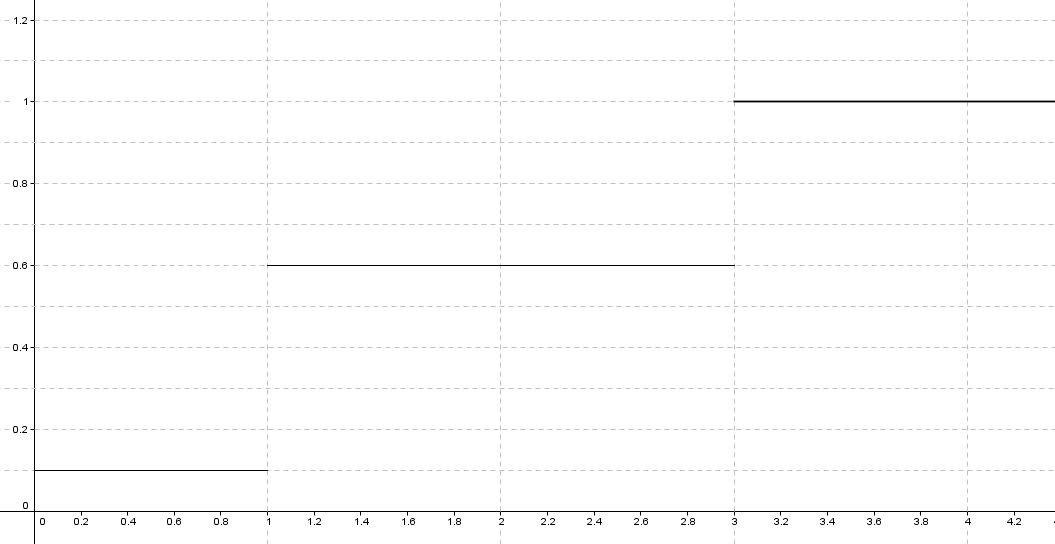
\includegraphics[scale=0.5]{Graph1.png}
\newline
ne vous amusez pas à dessiner des escaliers, cela peut vous être compter faux car on ne peut avoir de graphe vertical.

Maintenant supposons que X est une v.a discrète tel que 
\begin{eqnarray}
P(X=x) = f(x) = \left \{
\begin{array}{r c l}
0.1 x \text{ si 0$\leq x <4.5$} \\
0 \text{ sinon} \\
\end{array}
\right . 
\end{eqnarray}
\newline
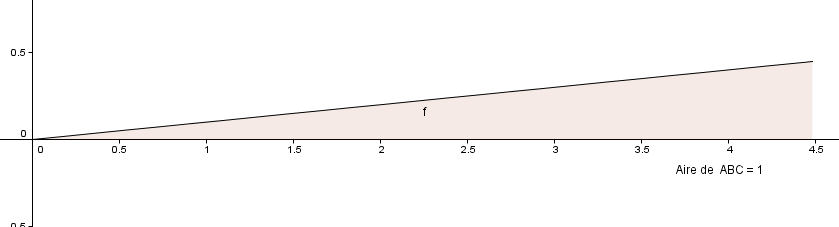
\includegraphics[scale=0.5]{Graph2.png}
\newline
Si je veux $P(X \leq 2)$ il faut que je calcul la somme de de tous les $f(i) = P(X=i)$ pour i inférieur à 2. Cela donne en fait l'aire entre la droite et l'axe x sur [0,2]
\newline
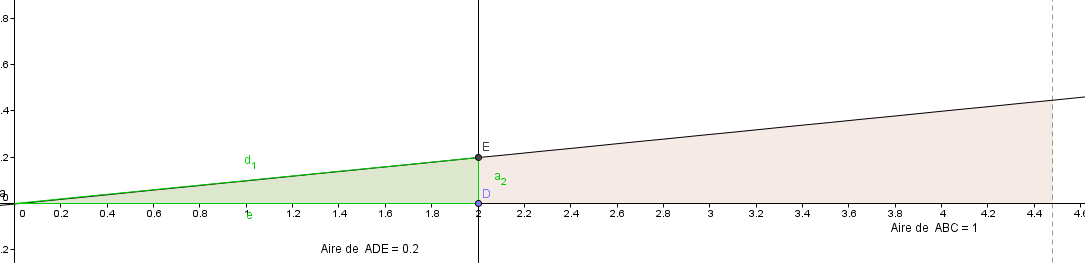
\includegraphics[scale=0.5]{Graph3.png}
\newline
Ce qui nous fais 0.2
\newline Ainsi pour calculer $P(X\leq x)$ quand x est inférieur à 4.5, il faut calculer l'intégrale sur [0,x], donc de $0.1x$,  ce qui nous donne ici $0.1x^2/2$. Puis sur [$-\infty$,0] ce qui nous donne 0 car la primitive de 0 c'est 0. On utilise alors la \textbf{relation de Chasle} qui consiste à additionner les différents aires sur [$-\infty$,x] (en somme, tout ce qui est inférieur à x) donc $P(X\leq x) = 0 \text{(integrale de f sur [$-\infty$,0])} + (F(x) - F(0)) \text{(integrale de f sur [0,x])} = 0 + 0.1 * x^2 /2 - 0.1 * 0 / 2 = 0.1 * x^2/2 \Leftrightarrow P(X \leq 2) = 0.2$ Donc \newline
\begin{eqnarray}
P(X\leq x) = F(x) = \left \{
\begin{array}{r c l}
0 \text{ si x$\leq 0$} \\
0.1 * x^2 / 2  \text{si $0<x \leq 2$} \\
1 \text{ sinon}
\end{array}
\right . 
\end{eqnarray}
\newline
Maintenant supposons que je souhaite avoir la probabilité que X soit entre 1 et 3.5. Ce qu'il faut que je fasse c'est calculer tout ce qu'il y a avant 3.5, donc avec la fonction de répartition qu'on a déterminé juste avant on calcul $F(3.5)$, puis on enlève ce qu'il y a avant 1, donc $F(1)$ et il nous restera que la partie qui nous intéresse. \newline
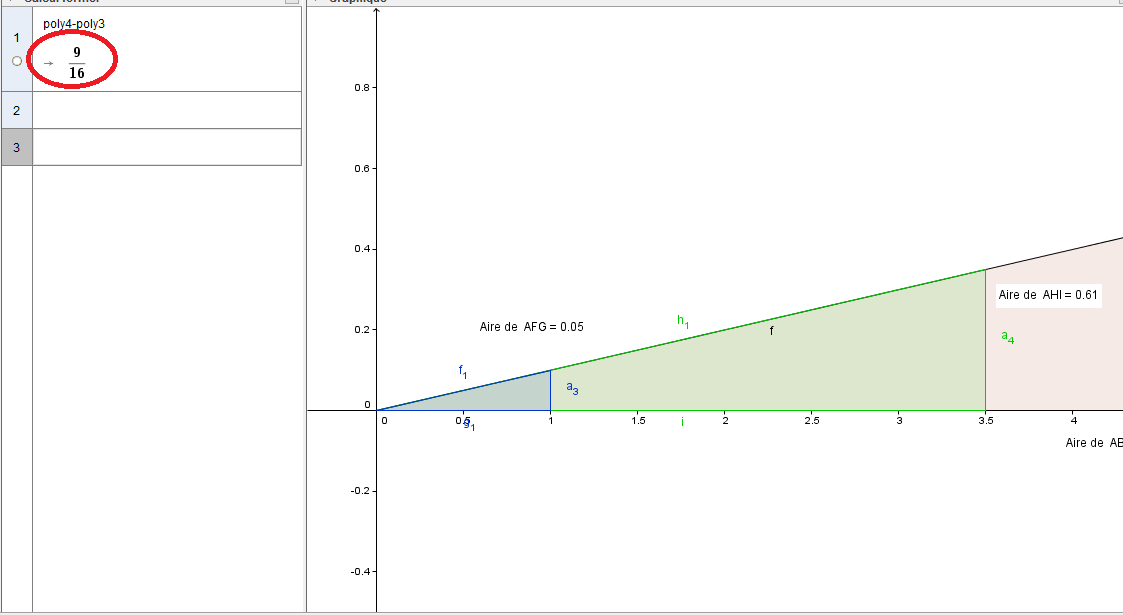
\includegraphics[scale=0.6]{Graph4.png}
\newline

\textbf{Propriété :} La fonction de répartition d'une variable discrète X tel que f(x) = P(X=x) est la primitive de la fonction f dans si et seulement si, à l'intérieur des bornes dans laquelle elle est définis :
\begin{itemize}
\item f et continue à l'intérieur des bornes dans laquelle elle est définis
\item f est positif 
\item L'intégrale de f, de sa borne inférieur à sa borne supérieur, est égale à 1
\end{itemize} 
On dit alors que X est une v.a continue et que f est sa densité de probabilité ($\neq$ fonction de répartition)
Dans notre exemple, la fonction f est continue et positif sur [$-\infty , +\infty$] et 
$$ \int_{-\infty}^{+\infty} f(t)\text{d}t = li - F(0) = 1 $$
donc f(x) est la densité de probabilité de X. \textbf{Attention}, sa fonction de répartition n'est pas 

\subsection{Couple de variable Aléatoire}

La loi du couple des variables aléatoires X,Y est la loi $P_{XY}$ tel que $P_{XY}({(x,y)})$ soit la probabilité que X soit égale à x et Y soit égale à y. On le note plus communément $P(X=x \bigcap Y=y)$. \newline
\textbf{Exemple :} Le couple (X,Y) suit la loi suivante : \newline
\begin{tabular}{|c|c|c|c|}
\hline
x / y & 0 & 1 & P(X = x)\\
\hline
0 & \textcolor{Blue}{0.3} & 0.1 & 0.4\\
\hline
1 & 0.15 & 0.2 & 0.35 \\
\hline
2 & 0.1 & 0.15 & \textcolor{Green}{0.25}\\
\hline
P(Y=y) & \textcolor{Red}{0.55} & 0.45 & 1\\
\hline
\end{tabular}
\newline
J'ai ici utilisé la formule des probabilités totales pour calculer la ligne P(Y=y) et la colonne P(X=x).
\begin{itemize}
\item La case blue est la probabilité $P(X=0 \bigcap Y=0)$. 
\item La case verte est la probabilité $P(X=2)$. 
\item La case rouge est la probabilité $P(Y=0)$. 
\end{itemize}

\subsection{Propriété de Variable aléatoire}
\subsubsection{Espérance}
L'espérance représente la valeur moyenne que l'on peut obtenir. Par exemple si je lance un dé et que j'associe la variable X à la valeur que me donnera le dé. L'espérance de X sera 3.5 et non pas 3 car on ne peut pas obtenir 0. L'espérance se calcul de la façon suivante :
$$ \sum_i xi * pi $$ \newline
Et ouais... pas assez explicite? bon d'accord. Il faut faire multiplier chaque valeur possible avec sa probabilité d'obtention, puis faire la somme de tous ces produit.
\newline \textbf{Exemple} : Dans le cas du lancé de dé, chaque valeur a $\frac{1}{6}$ chance de tomber. Ainsi pour obtenir l'espérance je fais $ E(X) = \frac{1}{6} * 1 + \frac{1}{6} * 2 + \frac{1}{6} * 3 + \frac{1}{6} * 4 + \frac{1}{6} * 5 + \frac{1}{6} * 7 = 3.5$ 
\newline
L'espérance d'un couple E(XY) se calcul de la même façon, pour chaque combinaison (i,j) possible il faut multiplier i, j et $P(X=i \bigcap Y=j)$ puis en faire la somme.
\newline
L'espérance est une fonction linéaire, ce qui veut dire entre-autre que si a et b sont deux constantes alors E(aX + b) = aE(X) + b
\newline
Pour une variable à densité il faut calculer l'espérance en calculant l'intégrale de x * f(x) sur $-\infty$ à $+\infty$. $$ E(X) =  \int_{-\infty}^{+\infty} t * f(t)\text{d}t$$

\textbf{Note} : On peut aussi dire de l'espérance qu'il y a autant de probabilité d'avoir moins de l'espérance que d'avoir plus : $P(X \leq E(x)) = P(X \geq E(x))$. Ainsi je peux dire que la X est centrée en X. 


\subsubsection{Variance et Ecart type}
 
 La variance indique de quelle manière la variable aléatoire se disperse autour de son espérance. Une variance égale à zéro montre que toutes les valeurs sont identiques. Une petite variance indique que les valeurs sont proches les unes des autres alors qu'une variance élevée montre le contraire.
 
 Elle se calcul avec la formule $V(X) = E(X^2) - E(X)^2$\newline
 Si on prend deux constante a et b alors $V(aX+b) = a^2 V(X)$ \newline
 \textbf{Note} : La variance est toujours positifs, si vous trouvez quelque chose de négatifs, remettez en doute votre calcul. \newline
 l'écart type $\sigma$ est tout simplement la racine de la variance.
 \subsubsection{Covariance et Corrélation}
 
 La covariance est, comme je l'aime l'appelé, la variance d'un couple. Elle se calcule de la façon suivante   $cov(XY) = E(XY) - E(X)E(Y)$ ainsi la covariance d'un couple (X,X) est la variance de X. \newline
 Si la covariance est non nul, alors X et Y sont \textbf{corrélées}.
 S'ils sont corrélées alors leur coefficient de corrélation est non nul et égale à $\rho (X,Y) =\frac{cov(X,Y)}{\sigma (X)x\sigma (Y)}$ \newline
 Si deux variable aléatoire sont indépendante alors elle sont non corrélées. la réciproque n'est pas toujours vrai. \newline
 \textbf{Note} : Si on vous demande si deux variable aléatoire sont indépendante puis d'en déduire s'ils sont corrélées alors elles sont forcément indépendante. Vous pouvez donc en déduire qu'elles sont corrélées.
 \textbf{Note 2} : Le coefficient de corrélation est compris entre 1 et -1. De plus $\rho (X,Y) = 1 ou -1 \Leftrightarrow Y = aX + b$ où a et b sont des réels fixés.
\subsection{Loi usuelle}
Les lois usuelles sont des lois qui sont appliqués à une certaine situation et sont définis par certaines règles.
\subsubsection{Loi uniforme}
X suit une loi uniforme de paramètre $| \Omega |$ si pour tout x de l'ensemble $\Omega$, on a alors $P(X=x)=frac{1}{|\Omega |}$. \newline
\textbf{Paramètres}
$E(X) = \frac{n+1}{2}$ et $ V(X)=\frac{n^2-1}{12}$ \newline
Il s'agit d'une loi à densité si $\Omega$ est un ensemble fini et continue (d'un réel a à un réel b). La densité de probabilité de X est alors 
\begin{eqnarray}
f(x) = \left \{
\begin{array}{r l l}
\frac{1}{b-a} \text{ si $x \in \Omega$} \\
0 \text{ sinon} \\
\end{array}
\right . 
\end{eqnarray} et sa fonction de répartition est 
\begin{eqnarray}
F(x) = \left \{
\begin{array}{r l l}
0 \text{ si x < a} \\
\frac{x-a}{b-a} \text{ si $x \in [a,b]$} \\
1 \text{ sinon} \\
\end{array}
\right . 
\end{eqnarray}
\subsubsection{Loi de Bernoulli}
X suit une loi de Bernoulli de paramètre p si X ne peut que prendre les valeur 1(réussite) et 0(échec). p étant la probabilité de réussite. \newline
\textbf{Paramètres}
$E(X) = p$ et $ V(X)=p(1-p)$
\subsubsection{Loi Binomiale}
X suit une loi Binomiale de paramètre (n,p) si X représente le nombre de réussite dans une suite d'épreuves de Bernoulli identique \textbf{effectué dans les mêmes conditions / avec remise}, on a alors $P(X=x)=\left( \begin{array}{l} n \\ p \end{array} \right) p^x (1-p)^(n-x)$. p étant la probabilité de réussite et n le nombre d'expérience. \newline
\textbf{Paramètres} 
$E(X) = np$ et $ V(X)=np(1-p)$
\subsubsection{Loi Hypergéométrique}
X suit une loi Hypergéométrique de paramètre (N,n,p) si X représente le nombre de réussite dans une suite d'épreuves de Bernoulli \textbf{dont chaque épreuve dépend des précédentes / sans remise}, on a alors $P(X=x)=\frac{\left(M \\ x \right) \left(N - M \\ n - x \right)}{\left(N \\ n \right)} $. p étant la probabilité de réussite lors de la première expérience, n le nombre d'expérience et N la proportion de réussite.\newline
\textbf{Exemple} : Une boite contient M boules dont N boules blanche. Je tire n à la suite boules sans les remettre. X est le nombre de boules blanche que j'ai tirée. X suit alors la loi hypergéométrique de paramètre (N,n,N/M) \newline

\textbf{Paramètres}
$E(X) = np$ et $ V(X)=\frac{np(1-p)(N-n)}{N-1}$
\subsubsection{Loi Géométrique}
X suit une loi Géométrique de paramètre p si X représente le nombre d'épreuve qu'il faut pour une obtenir une réussite dans une itération d'épreuves de Bernoulli identique, on a alors $P(X=x)=p * (1-p)^{x-1} $. p étant la probabilité de réussite.\newline
\textbf{Exemple} : Une boite contient des boules et la chance d'obtenir une boule blanche est p. Je prends les boules sans les remettre tant que je n'ai pas pris de boule blanche. X est le nombre de boules que j'ai tirée avant d'obtenir une boule blanche. X suit alors la loi géométrique de paramètre p \newline

\textbf{Paramètres}
$E(X) = \frac{1}{p}$ et $ V(X)=\frac{1-p}{p^2}$

\textbf{Note} : Sachant que j'ai tiré n boules, les probabilités que je prennent une boule blanche au bout de k autres épreuves est la même que lorsque j'ai tiré la première boule. Cette propriété de la loi Géométrique le définis en tant que loi \textbf{sans vieillissement (ou loi sans mémoire)} : $P(X> n + k | X>n) = P(X>k)$.
\subsubsection{Loi Normal}

\textbf{Cas Particulier : Loi Normal centré réduite}
\newline
Une loi est centré lorsque son espérance \textbf{$\mu$} est égale à 0, petit rappel, cela veut dire qu'on a autant de chance de tombé en dessous de 0 qu'au dessus. Elle est réduite quand l'écart type \textbf{$\sigma$} est égale à 1. Cela veut dire que X ne varie pas énormément, mais ne vous souciez pas de ce que ça veut dire. On dit que X suit la loi N(0,1), la loi normal d'espérance 0 et d'écart type 1( centré réduite).
\newline
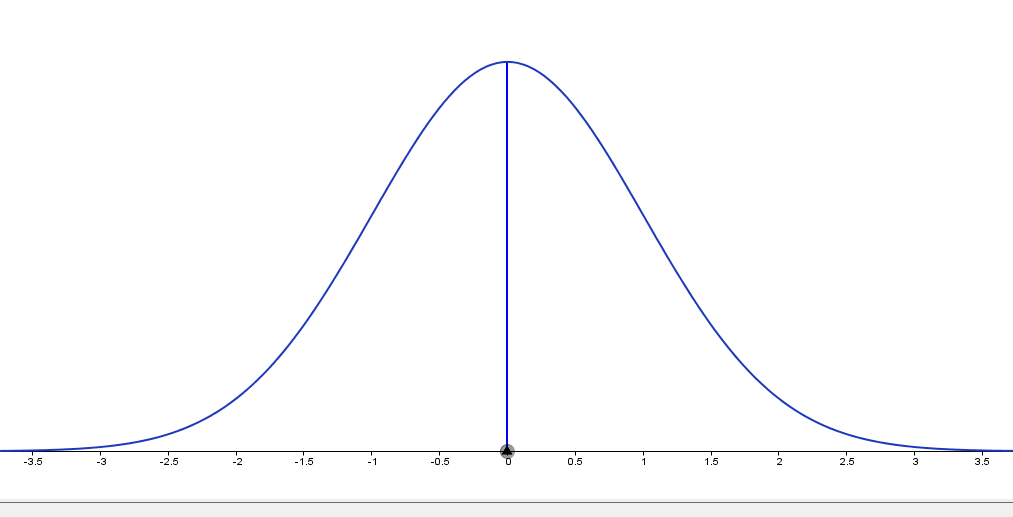
\includegraphics[scale=0.6]{Graph5.png}
\newline
La fonction de répartition de la Loi Normal est $\Phi (x)$, dont le calcul ne vous ai pas demandé car certaines personne ont eu la bonne idée de mettre les résultats dans un tableau pages 42 \textbf{et} 43 de votre formulaire. Je ne vais pas vous apprendre à l'utiliser parce que ça m'obligerai à tout retaper, donc  je vous donne un pitit exemple et vous vous débrouillerai :
\textbf{Exemple }:
X suit la loi Normal centré réduite. Quelle est la probabilité quelle soit inférieur à 1.27? \newline
Dans le tableau je prend la ligne où se trouve 1.20 puis la colonne où se trouve 0.07 (1.27 = 1.20 +0.07) et je trouve mon résultat.
\textbf{Exemple 2 }:
X suit la loi Normal centré réduite. Quelle est la probabilité quelle soit inférieur à -1? \newline
Dans le tableau je prend la ligne où se trouve -1... zut! j'ai pas la ligne -1 T.T... Il faut dans ce cas exprimer le calcul de sorte à ce que l'expression contiennent une probabilité qu'on connaisse. 
\newline
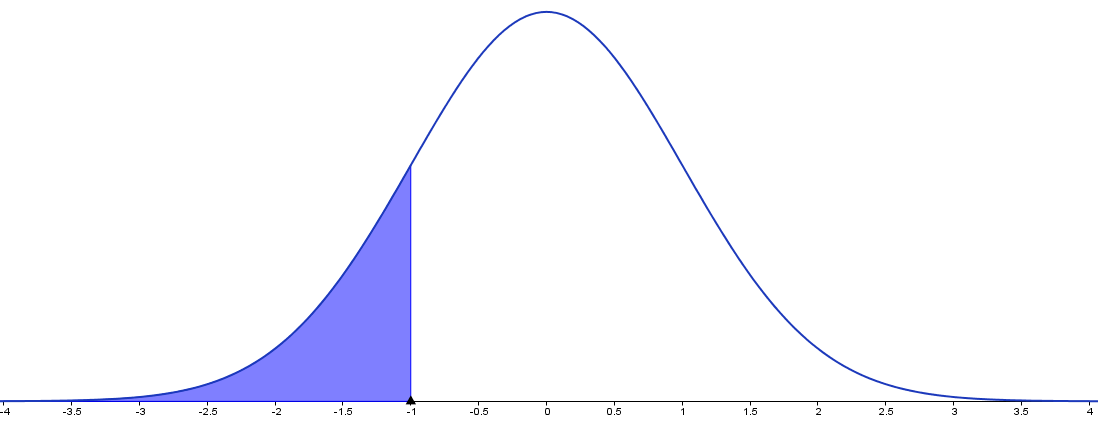
\includegraphics[scale=0.6]{Graph6.png}
\newline
\textbf{Note} : Puisque la loi est centré alors : $P(X<-x) = P(X>x)$
\newline
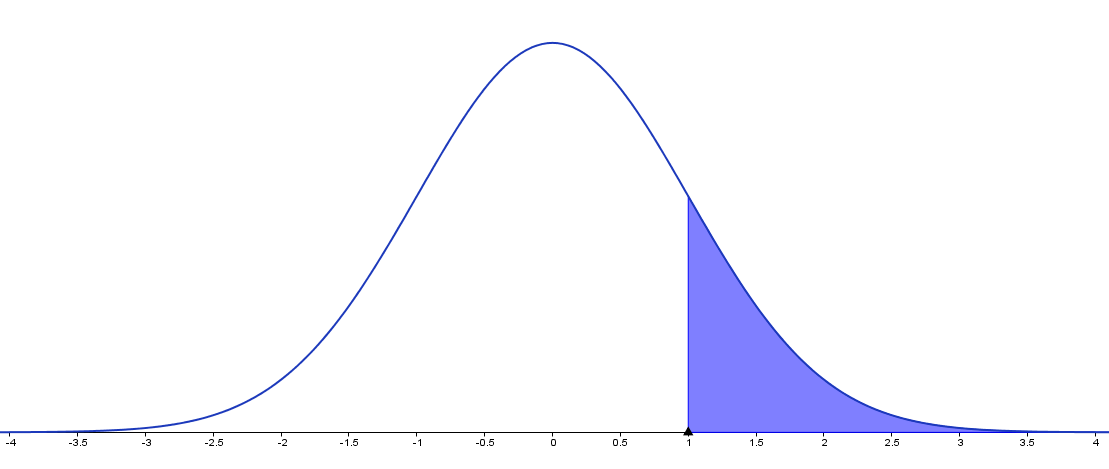
\includegraphics[scale=0.7]{Graph7.png}
\newline
Marrant n'est ce pas? Mais ne foncez pas sans réfléchir! \underline{$\Phi (-x) \neq \Phi (x)$}, $\Phi (x) =$ \newline
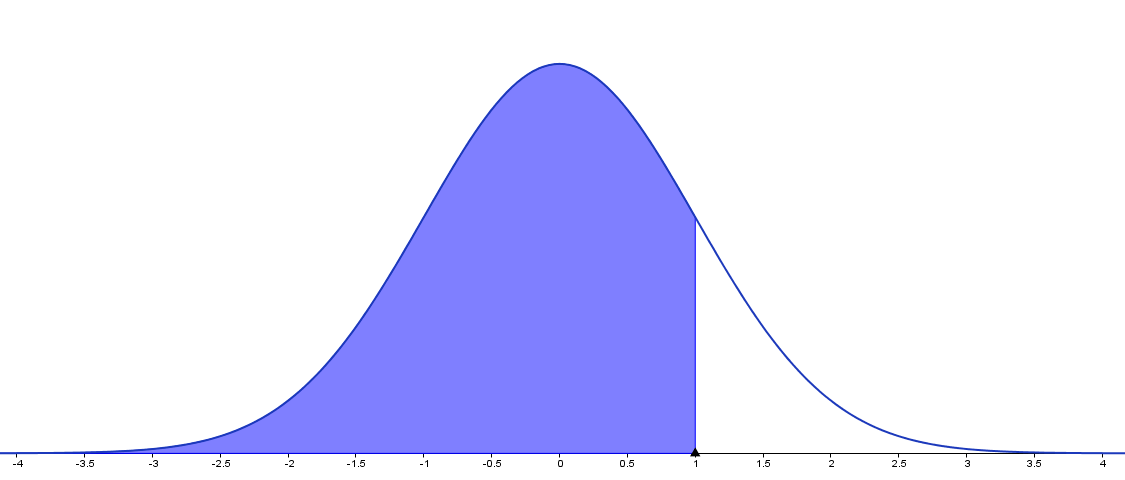
\includegraphics[scale=0.7]{Graph8.png}
\newline
Étant donnée que nous voulons le reste il faut faire $\Phi (-x) = 1 - \Phi (x)$ ce qui nous donne $\Phi (-1) = 1 - \Phi (1) = 1 - 0.8413 = 0.1587$
\newline
\textbf{Cas Général : Loi Normal quelconque}
\newline
Si X suit la loi Normal d'espérance $\mu$ et d'écart type $\sigma$ alors $X = \sigma X^* + \mu$ où $X^*$ suit la loi Normal centré réduite. Ce qui implique que $P(X<x) = P(\sigma X^* + \mu < x) \Leftrightarrow P(X<x) = P(X^* < \frac{x - \mu}{\sigma}) = \Phi (\frac{x - \mu}{\sigma})$. Pourquoi tout cela? Parce que tout simplement je sais calculer $\Phi (\frac{x - \mu}{\sigma})$ ce qui n'est pas le cas pour $P(X<x)$. J'aimerai vous montrer une erreur disant \underline{conséquente} (Dédicaces à M. Bensadon) : $P(X<x) = P(\sigma X + \mu < x)$, ceci est faux. Pensez bien à changer de variable aléatoire en spécifiant que $X^*$ suit la loi N(0,1).

\textbf{Note importante} : Cette note est importante car elle concerne l'exercice "qui n'a pas été noté" lors de la dernière interrogation, ce qui implique qu'il peut venir vous dire un petit coucou au DS. Notons $X1 \sim N(\mu 1, \sigma 1)$ (suivant la loi normal d'espérance $\mu 1$ et d'écart type $\sigma 1$) et $X2 \sim N(\mu 2, \sigma 2)$, si X1 et X2 sont indépendantes entre eux alors $X1+X2 \sim N(\mu 1 + \mu 2, \sqrt{\sigma 1^2\sigma 2^2})$. \newline
Notons une suite de n v.a indépendantes et identiques suivant la même loi normal. $\frac{1}{n} \sum_{i=1}^n \sim N(\mu, frac{\sigma}{\sqrt{n}})$

\subsubsection{Loi du khi-deux}
Qui ça? le maharadja ofc. J'aimerai apporté une correction aux formulaire. Notons une suite de n v.a indépendantes et identiques suivant tous loi normal centré réduite. La variable $Y = \sum_{i=1}^n X_i^2$ suit la loi de khi-deux de n degrés de liberté. Et non pas $Y = \sum_{i=1}^n X_{i^2}$. \newline
Bref à quoi sert ce charabia? Elle sert à déterminer la densité de probabilité, dont je ne vais m'amuser à réécrire les formules, et à déterminer l'espérance $E(Y)= n$ et la variance $V(Y)= 2n$

\subsubsection{Autre Loi}
Pour les autres lois, je vous laisse regarder le formules.

\subsection{Convergence et approximation}

\subsubsection{Approximation}
L'approximation d'une loi L1 avec une autre L2 permet de calculer une probabilité en se basant sur la loi L2. C'est assez bête n'est ce pas? En fait, le tableau que vous retrouvez à la page 34 résume bien ce que vous devez savoir pour l'approximation. Vous devez validé les conditions pour affirmer qu'une loi peut être approximer par une autre.

\subsubsection{Convergence et TLC}
On dit que $X_n$, suivant une loi qui dépend de n, converge en Loi vers X si $\lim_{n\leftarrow +\infty}  F_n(x) = F(x) $ avec $F_n$ la fonction de répartition de $X_n$ et $F$ la fonction de répartition de X. On note alors, $Xn \leftarrow^L X$
\textbf{théorème de limite centrale} : Vu que j'arrive vers la fin de la partie "Variable Aléatoire", je n'ai pas vraiment envie de vous réécrire bêtement ce que le formulaire explique très bien. Je vous redirige donc vers la page 32 de votre formulaire. Toutefois ne négligé pas cette partie.

\section{Chaine de Markov}

Vu que j'aime bien l'exemple de M. Bensadon, je vais le reprendre. Voici la situation de Bubulle le poisson rouge.
\newline
\noindent
\includegraphics[scale=0.8]{Bubulle le poisson rouge.jpg}
\newline
Vu ainsi, ce graphe doit être incompréhensible, pourtant il est très simple. Ce graphe présente 3 états de Bubulle numéroté de 1 à 3.
\begin{enumerate}
\item Dormir
\item manger
\item tourner dans son bocale
\end{enumerate}
Pour chaque états, Bubulles peut faire autre chose, ce changement d'état est représenté par une flèche. Les valeurs correspondant aux flèches représente la probabilité que Bubulle passe de léetat source à l'état destination. Par exemple la flèche partant de 1 et allant à 3 représente le changement de l'état "Bubulle dort" à l'état "Bubulle mange" et "0.7" est la probabilité que Bubulle mange après avoir dormis.
La chaîne de Markov est la suite de variable aléatoire $(X_n)_{n \in \mathbb{N}}$, dont chaque $X_i$ est égale à l'état de Bubulle à l'instant i. 
\textbf{La matrice de transition} associé à ce graphe est une matrice carrée dont chaque coefficient $x_{ij}$ correspond à la probabilité de passé de l'état i à l'état j.
\newline
\begin{eqnarray}
\begin{array}{l c r c c}
1 & 2 & 3 & &
\end{array} \\
\left.
\begin{array}{l}
1 \\
2 \\
3
\end{array}
 \right.
 \left(
\begin{array}{c c c}
0.1 & 0.2 & 0.7 \\
0.8 & 0 & 0.2 \\
0.2 & 0.6 & 0.2
\end{array}
 \right)
\end{eqnarray}

La matrice $P(i)$ est la matrice colonne dont chaque coefficient représente chacun des probabilités que Bubulle soit dans un état spécifique à l'instant i. 
\newline
\textbf{Exemple} : $P(0)=\left( \begin{array}{c} P(X_0=1) \\ P(X_0=2) \\ P(X_0=3) \end{array} \right)= \left( \begin{array}{c} 0.2 \\ 0.4 \\ 0.4 \end{array} \right)$. Il s'agit de l'état initial de Bubulle. A partir de cet matrice on peut déterminer les probabilité suivante. \newline
\textbf{Note} : La chaine de Markov suit une loi sans vieillissement, donc P(i) ne dépend que de P(i-1). La corrélation entre ces deux probabilités est $P(i) = ^tM * P(i-1)$. On dit alors que la matrice de transition est \textbf{homogène} car elle dépend d'aucune variable. \newline
\textbf{Note} : La matrice de transition est \textbf{une matrice stochastique} car la somme des coefficient sur une ligne/colonne est égale à 1.
\textbf{Une Loi est stationnaire} si d'un instant i à un instant i+1 les probabilités restent les mêmes. $P(i) = P(i+1)$


\end{document} 